\documentclass[../main.tex]{subfiles}

\begin{document}

\chapter{Results}

\section{Maintainability Cost Evaluation Results}

\subsection{Graylog}

\begin{table}[H]
    \centering
    \begin{tabular}{|c|c|c|c|c|c|c|}
        \hline
    \textbf{\shortstack{Helm \\ Chart \\ Version }} & \textbf{\shortstack{Update \\ Time 1 \\ (in seconds)}} & \textbf{\shortstack{Update \\ Time 2 \\ (in seconds)}} & \textbf{\shortstack{Update \\ Time 3 \\ (in seconds)}} & \textbf{\shortstack{Smoke \\ Test}} & \textbf{\shortstack{Upgraded \\ App}} & \textbf{\shortstack{Manual \\ Inter- \\ vention}} \\
        \hline
        2023-02-14 & 196.23 & 254.41 & 195.34 & + & Graylog & - \\
        2023-02-28 & 449.95 & 461.32 & 448.65 & + & OpenSearch & - \\
        2023-03-01 & 193.75 & 196.81 & 196.66 & + & Graylog & - \\
        2023-03-06 & 196.62 & 196.36 & 193.56 & + & Graylog & - \\
        2023-03-14 & 43.25 & 42.39 & 40.32 & + & MongoDB & - \\
        2023-04-05 & 197.38 & 197.03 & 194.18 & + & Graylog & - \\
        2023-05-03 & 439.89 & 451.40 & 439.52 & + & OpenSearch & - \\
        2023-05-11 & 194.96 & 196.88 & 194.38 & + & Graylog & - \\
        2023-05-12 & 39.09 & 41.91 & 39.35 & + & MongoDB & - \\
        2023-05-25 & 193.35 & 196.13 & 192.07 & + & Graylog & - \\
        2023-06-06 & 438.93 & 448.35 & 436.62 & + & OpenSearch & - \\
        2023-06-07 & 193.26 & 195.01 & 193.54 & + & Graylog & - \\
        2023-07-01 & 40.99 & 42.25 & 40.87 & + & MongoDB & - \\
        2023-07-05 & 193.28 & 196.25 & 195.71 & + & Graylog & - \\
        2023-07-15 & 38.97 & 41.63 & 39.64 & + & MongoDB & - \\
        2023-07-25 & 437.54 & 440.35 & 479.45 & + & OpenSearch & - \\
        2023-08-02 & 195.78 & 194.13 & 194.20 & + & Graylog & - \\
        2023-08-25 & 41.29 & 40.15 & 41.21 & + & MongoDB & - \\
        2023-09-06 & 195.76 & 194.78 & 193.06 & + & Graylog & - \\
        2023-09-14 & 41.45 & 41.91 & 41.65 & + & MongoDB & - \\
        2023-09-25 & 439.60 & 441.12 & 469.85 & + & OpenSearch & - \\
        2023-10-04 & 193.81 & 196.56 & 197.46 & + & Graylog & - \\
        2023-10-12 & 196.90 & 196.55 & 194.97 & + & Graylog & - \\
        2023-10-16 & 449.49 & 450.49 & 478.05 & + & OpenSearch & - \\
        2023-11-01 & 194.65 & 195.71 & 195.75 & + & Graylog & - \\
        2023-11-15 & 193.77 & 193.35 & 193.67 & + & Graylog & - \\
        2023-12-01 & 439.65 & 449.06 & 499.40 & + & OpenSearch & - \\
        2023-12-06 & 193.06 & 193.40 & 195.04 & + & Graylog & - \\
        \hline
    \end{tabular}
    \caption{Installation and Upgrade Data}
    \label{tab:graylog_results_2023}
\end{table}


\begin{table}[H]
    \centering
    \begin{tabular}{|c|c|c|c|c|c|c|}
        \hline
        \textbf{\shortstack{Helm \\ Version}} & \textbf{\shortstack{Update \\ Time 1 \\ (in seconds)}} & \textbf{\shortstack{Update \\ Time 2 \\ (in seconds)}} & \textbf{\shortstack{Update \\ Time 3 \\ (in seconds)}} & \textbf{\shortstack{Smoke \\ Test}} & \textbf{\shortstack{Upgraded \\ App}} & \textbf{\shortstack{Manual \\ Inter- \\ vention}} \\
        \hline
        2024-01-03 & 195.30 & 195.52 & 200.84 & + & Graylog & - \\
        2024-02-07 & 195.40 & 196.35 & 196.96 & + & Graylog & - \\
        2024-02-21 & 470.66 & 471.58 & 500.99 & + & OpenSearch & + \\
        2024-03-06 & 196.77 & 196.72 & 195.73 & + & Graylog & - \\
        2024-04-03 & 469.80 & 458.52 & 520.72 & + & Graylog, OpenSearch & - \\
        2024-04-17 & - & - & - & - & Graylog & - \\
        2024-04-27 & - & - & - & - & MongoDB & - \\
        2024-05-13 & - & - & - & - & Graylog & - \\
        2024-05-15 & - & - & - & - & OpenSearch & - \\
        2024-05-22 & - & - & - & - & Graylog & - \\
        2024-05-28 & - & - & - & - & Graylog & - \\
        2024-06-05 & - & - & - & - & Graylog & - \\
        2024-06-26 & - & - & - & - & OpenSearch & - \\
        2024-07-01 & - & - & - & - & MongoDB & - \\
        2024-07-03 & - & - & - & - & Graylog & - \\
        2024-08-07 & - & - & - & - & Graylog & - \\
        2024-08-27 & - & - & - & - & MongoDB & - \\
        2024-09-04 & - & - & - & - & Graylog & - \\
        2024-10-02 & 471.95 & 502.58 & 480.34 & + & Graylog & - \\
        2024-10-12 & 200.23 & 198.78 & 198.86 & + & Graylog & - \\
        2024-10-23 & 199.96 & 197.52 & 197.03 & + & Graylog & - \\
        2024-11-06 & 199.35 & 194.62 & 196.94 & + & Graylog & - \\
        2024-11-21 & 200.08 & 196.85 & 194.88 & + & Graylog & - \\
        2024-12-04 & 197.26 & 196.82 & 196.69 & + & Graylog & - \\
                \hline
    \end{tabular}
    \caption{Installation and Upgrade Data}
    \label{tab:graylog_results_2024}
\end{table}

\subsection{Graylog Major Updates Only}

\begin{table}[H]
    \centering
    \begin{tabular}{|c|c|c|c|c|c|c|}
        \hline
        \textbf{\shortstack{Helm \\ Version}} & \textbf{\shortstack{Update \\ Time 1 \\ (in seconds)}} & \textbf{\shortstack{Update \\ Time 2 \\ (in seconds)}} & \textbf{\shortstack{Update \\ Time 3 \\ (in seconds)}} & \textbf{\shortstack{Smoke \\ Test}} & \textbf{\shortstack{Upgraded \\ App}} & \textbf{\shortstack{Manual \\ Inter- \\ vention}} \\
        \hline
        2023-02-28 & 475.97 & 496.12 & 528.47 & + & OpenSearch & - \\
        2023-05-03 & 504.90 & 506.06 & 496.57 & + & OpenSearch & - \\
        2023-05-11 & 192.37 & 192.00 & 193.93 & + & Graylog & - \\
        2023-06-06 & 487.12 & 456.28 & 477.22 & + & OpenSearch & - \\
        2023-07-25 & 497.12 & 484.46 & 507.63 & + & OpenSearch & - \\
        2023-09-25 & 494.62 & 476.18 & 477.58 & + & OpenSearch & - \\
        2023-10-16 & 476.62 & 496.08 & 478.33 & + & OpenSearch & - \\
        2023-11-01 & 192.82 & 192.27 & 193.26 & + & Graylog & - \\
        2024-02-21 & 486.54 & 506.41 & 547.98 & + & OpenSearch & + \\
        2024-04-03 & 496.44 & 496.30 & 498.12 & + & Graylog, OpenSearch & - \\
        2024-04-17 & - & - & - & - & Graylog & - \\
        2024-04-27 & - & - & - & - & MongoDB & - \\
        2024-05-15 & - & - & - & - & OpenSearch & - \\
        2024-06-26 & - & - & - & - & OpenSearch & - \\
        2024-10-12 & 497.04 & 506.61 & 509.61 & + & Graylog & - \\
        \hline
    \end{tabular}
    \caption{Installation and Upgrade Data}
    \label{tab:graylog_results_2024}
\end{table}

\subsection{Logging Operator}

The table~\ref{table:logging_operator_results} displays the update times for the Logging Operator. These times represent the duration (in seconds) taken for the first installation and subsequent updates across 3 different trials.

Additionally, the table includes two columns: "Smoke Test" and "Manual Intervention". The "Smoke Test" column indicates whether the software passed its basic functionality check after installation (with "+" meaning pass, and "-" meaning fail). The "Manual Intervention" column shows whether any manual adjustments were needed during the installation process (with "+" indicating that intervention was required and "-" meaning no intervention was necessary).

All updates were successful, with an average installation time of 7.39 seconds. Notably, no manual intervention was required for any of the updates. While some versions, such as Version 4.9.0, stand out with much longer installation times, or some versions, like Version 4.11.2, take longer during some trials than others, all updates were completed in under one minute, demonstrating efficient performance across all versions.

\begin{table}[ht]
    \centering
    \begin{tabular}{|c|c|c|c|c|c|}
    \hline
    \textbf{\shortstack{Helm Chart \\ Version}} & \textbf{\shortstack{Update \\ Time 1 \\ (in seconds)}} & \textbf{\shortstack{Update \\ Time 2 \\ (in seconds)}} & \textbf{\shortstack{Update \\ Time 3 \\ (in seconds)}} & \textbf{\shortstack{Smoke \\ Test}} & \textbf{\shortstack{Manual \\ Intervention}} \\
    \hline
    4.1.0 & 6,23 & 6,71 & 7,02 & + & - \\
    4.2.0 & 6,54 & 7,89 & 6,06 & + & - \\
    4.2.1 & 6,47 & 6,65 & 6,28 & + & - \\
    4.2.2 & 4,59 & 6,42 & 4,50 & + & - \\
    4.3.0 & 6,85 & 8,66 & 7,31 & + & - \\
    4.4.0 & 4,92 & 5,35 & 4,93 & + & - \\
    4.4.1 & 4,88 & 5,05 & 4,71 & + & - \\
    4.4.2 & 5,26 & 5,25 & 5,55 & + & - \\
    4.4.3 & 5,93 & 5,81 & 4,63 & + & - \\
    4.5.0 & 5,74 & 5,47 & 5,07 & + & - \\
    4.5.1 & 5,51 & 6,14 & 5,47 & + & - \\
    4.5.2 & 5,89 & 7,55 & 5,51 & + & - \\
    4.5.3 & 5,29 & 5,76 & 5,25 & + & - \\
    4.5.4 & 5,38 & 5,91 & 5,48 & + & - \\
    4.5.5 & 5,61 & 5,66 & 5,37 & + & - \\
    4.5.6 & 5,21 & 5,89 & 5,51 & + & - \\
    4.6.0 & 5,84 & 7,64 & 5,27 & + & - \\
    4.6.1 & 5,51 & 7,13 & 5,43 & + & - \\
    4.7.0 & 5,88 & 5,62 & 5,24 & + & - \\
    4.8.0 & 5,43 & 5,66 & 5,49 & + & - \\
    4.9.0 & 29,87 & 15,57 & 35,56 & + & - \\
    4.9.1 & 5,44 & 5,62 & 5,73 & + & - \\
    4.10.0 & 6,13 & 5,59 & 5,87 & + & - \\
    4.10.1 & 5,35 & 5,50 & 5,84 & + & - \\
    4.11.0 & 6,23 & 5,61 & 5,75 & + & - \\
    4.11.2 & 6,07 & 4,96 & 47,49 & + & - \\
    4.11.3 & 24,59 & 20,62 & 5,75 & + & - \\
    5.0.0 & 5,70 & 5,85 & 5,42 & + & - \\
    5.0.1 & 6,74 & 5,59 & 5,46 & + & - \\
    \hline
    \end{tabular}
    \caption{Installation Data}
    \label{table:logging_operator_results}
\end{table}

The installation script and table can be found in the Git repository https://gitlab.fisp.dev/Abdykalykova\_Z/logging\_operator/.

\subsection{Rancher Logging App}

The Rancher Logging App presents two versions \ref{fig:chart}: \texttt{104.1.0+up4.8.0} and \texttt{104.0.0+up4.4.0}. 
However, several problems arose during the installation.

\begin{figure}[H]
        \centering
        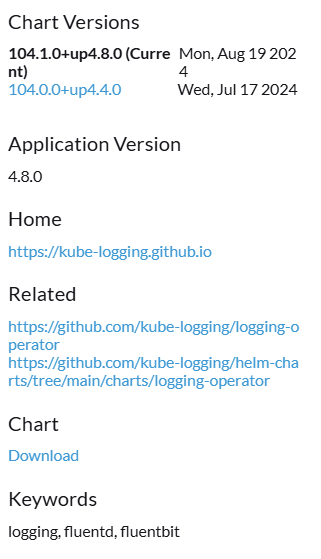
\includegraphics[]{img/5-results/chart.png}
        \caption{ }
        \label{fig:chart}
\end{figure}

On the test cluster, both installations were successful, but a known bug 
(https://github.com/rancher/rancher/issues/46862) was encountered. The Rancher team’s solution is to use a different Fluentd version. However, identifying this bug required manual effort and searching.  

On the dev cluster, the installation was unsuccessful, even though the same steps were followed as on the test cluster. Issues occurred with either Fluentd pods being stuck in a crash loop or Fluent Bit being unable to communicate with Fluentd. 

After manually searching for available images https://hub.docker.com/u/rancher, the latest versions were used, which finally led to a successful installation.

\begin{figure}[H]
        \centering
        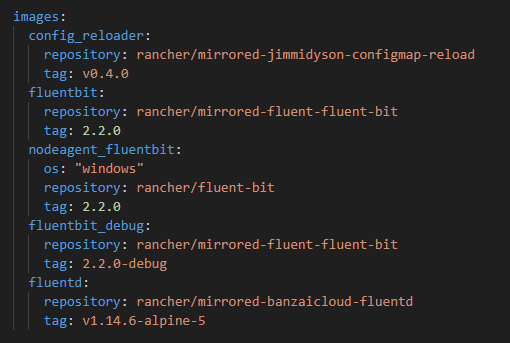
\includegraphics[]{img/5-results/values_images.png}
        \caption{ }
        \label{fig:values_images}
\end{figure}

\section{Productive Usage}

Introduction of Graylog as an internal service for all teams

If Graylog is provided centrally, it reduces the effort for each individual team. If Graylog is officially introduced as a central service, a technical owner must be assigned to be responsible for maintenance.

Current state:

The Kubernetes cluster runs in an in-house data center. Many different projects run on a shared clusters. Each project gets a namespace where they can install what they need. A transition to a new infrastructure is planned. In the future, teams will be able to create a dedicated cluster on demand. Currently, Rancher Logging and Graylog run internally on each cluster, and a ClusterOutput forwards logs to Graylog.

In the future, one/more (depends on demand) Graylog instance could still be provided centrally, with each cluster forwarding logs to an external URL. Rancher Logging will need to be installed on each cluster, which requires additional effort from teams. However, with a provided app „Rancher Logging“ in Rancher, the workload remains manageable, just installing the app by one click. The chart could be verified beforehand by technical application manager.

Internally, there is no 24/7 on-call support. While this is not an issue for internal applications, it could become relevant for a future production deployment for customers.

Applications can be upgraded either through CLI or directly though Rancher Apps that takes Helm charts from internal Git repository. Rancher \gls{ui} shows that App is upgradable as soon it is available, which can be installed per click. Since charts come from internal repository, no further modifications to values.yaml should be neccessary.

\begin{figure}[H]
        \centering
        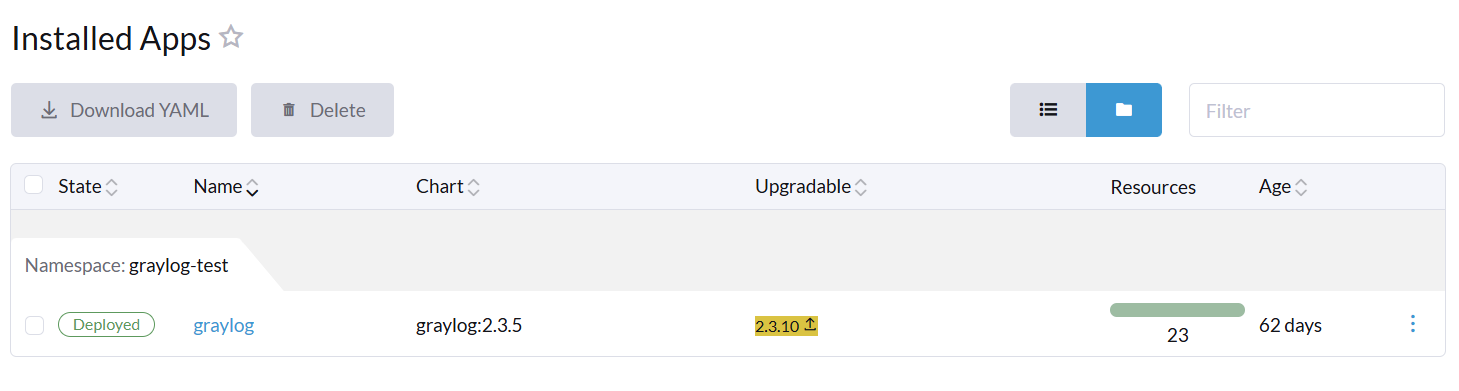
\includegraphics[scale=0.6]{img/3-background/rancher/rancher_update_graylog.png}
        \caption{Upgradable app on Rancher UI.}
        \label{fig:rancher_update_graylog}
\end{figure}

\subsection{Working with Application Logs: After the solution}

\subsection{Kano questioniere results}

https://de.wikipedia.org/wiki/Kano-Modell

\end{document}